% Requires in the preamble:
% \usepackage{amsmath,amssymb}
% \usepackage{tikz,pgfplots}
% \pgfplotsset{compat=1.18}

\chapter{Velocity, Distance, and the First Shape of Calculus}
\label{chap:velocity-distance}

A car dashboard already contains the first story of calculus. One instrument remembers how much road has been accumulated. Another tells how fast that accumulated amount is changing.

Those two ideas are not separate. They are inverse clues.

\[
\text{distance changes} \quad \longleftrightarrow \quad \text{velocity is measured},
\]
and
\[
\text{velocity is accumulated} \quad \longleftrightarrow \quad \text{distance changes}.
\]

Calculus begins by making this relation precise.

\section{The dashboard: speedometer and odometer}
\label{sec:dashboard}

Look at two instruments on a car dashboard.

The \emph{odometer} records distance. It tells how many miles the car has accumulated.

The \emph{speedometer} records speed. It tells how fast the odometer reading is changing.

For the moment, imagine that the car moves only forward along a straight road. Then speed and velocity agree. Later, when the car can reverse direction, we will need signed velocity.

\begin{figure}[h]
\centering
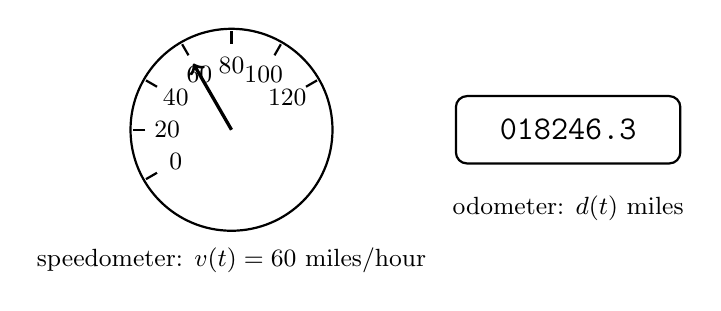
\begin{tikzpicture}[scale=0.95, every node/.style={font=\small}]
  % Speedometer
  \draw[thick] (0,0) circle (1.35);
  \foreach \ang/\lab in {210/0,180/20,150/40,120/60,90/80,60/100,30/120} {
     \draw[thick] ({1.15*cos(\ang)},{1.15*sin(\ang)})
       -- ({1.32*cos(\ang)},{1.32*sin(\ang)});
     \node at ({0.86*cos(\ang)},{0.86*sin(\ang)}) {\lab};
  }
  \draw[very thick,->] (0,0) -- ({1.02*cos(120)},{1.02*sin(120)});
  \node at (0,-1.75) {speedometer: \(v(t)=60\) miles/hour};

  % Odometer
  \draw[rounded corners,thick] (3.0,-0.45) rectangle (6.0,0.45);
  \node[font=\ttfamily\large] at (4.5,0) {018246.3};
  \node at (4.5,-1.05) {odometer: \(d(t)\) miles};
\end{tikzpicture}
\caption{The odometer records accumulated distance. The speedometer records how fast that distance is changing.}
\label{fig:dashboard}
\end{figure}

Let \(t\) denote time, measured in hours after the start of a trip. Let

\[
d(t)
\]

denote the number of miles traveled after \(t\) hours. Let

\[
v(t)
\]

denote the velocity at time \(t\), measured in miles per hour.

The notation \(d(t)\) means: the distance depends on the time. When the input is a time \(t\), the output is a distance \(d(t)\). We will soon give this kind of rule a name: a \emph{function}. For now, the notation lets us keep track of the trip.

\subsection{Distance as accumulated motion}

Suppose the odometer reads \(18{,}246.3\) miles at \(9{:}00\) and \(18{,}346.3\) miles at \(11{:}00\). During those two hours, the car has accumulated

\[
18{,}346.3-18{,}246.3=100
\]

miles.

The odometer does not say how the car traveled those \(100\) miles. The driver might have gone steadily. Or slowly at first and quickly later. The odometer remembers the total effect, not the moment-by-moment history.

If we reset the trip odometer at the start, then \(d(0)=0\). After \(2\) hours in this example,

\[
d(2)=100.
\]

The distance function \(d(t)\) is a memory of the trip.

\subsection{Velocity as changing distance}

Velocity measures how fast distance changes.

If the car travels \(100\) miles in \(2\) hours, then its \emph{average velocity} over that time is

\[
\frac{\text{change in distance}}{\text{change in time}}
=
\frac{100\text{ miles}}{2\text{ hours}}
=
50\text{ miles/hour}.
\]

Using \(d(t)\), this is

\[
\frac{d(2)-d(0)}{2-0}.
\]

This number is an average over an interval. It does not say that the car was moving at exactly \(50\) miles per hour at every instant. It only says that the total change, spread evenly over two hours, would be \(50\) miles per hour.

A speedometer asks a sharper question:

\[
\text{How fast is the distance changing right now?}
\]

That word ``right now'' is where calculus enters.

\subsection{Units already tell the story}

The units point to the mathematics.

\[
d(t) \quad \text{has units of miles},
\]
while
\[
v(t) \quad \text{has units of miles/hour}.
\]

So velocity must be built from distance divided by time. That is why ratios like

\[
\frac{d(b)-d(a)}{b-a}
\]

will appear again and again.

The numerator measures change in distance. The denominator measures change in time. Their quotient measures change per unit time.

\begin{center}
\begin{tabular}{c|c|c}
\textbf{symbol} & \textbf{meaning} & \textbf{units} \\ \hline
\(t\) & time after the start & hours \\
\(d(t)\) & distance traveled after \(t\) hours & miles \\
\(v(t)\) & velocity at time \(t\) & miles/hour
\end{tabular}
\end{center}

A good formula respects units. For example,

\[
\text{miles/hour}\cdot \text{hours}=\text{miles}.
\]

So multiplying velocity by time should produce a distance. This is exactly what happens when velocity is constant.

\subsection{The first question: distance to velocity}

Suppose we know the whole odometer record \(d(t)\). Can we recover the velocity \(v(t)\)?

For a long interval, we can compute only an average velocity. For example,

\[
\frac{d(2)-d(0)}{2}
\]

is the average velocity from time \(0\) to time \(2\).

To know the velocity near \(t=2\), we should look closer:

\[
\frac{d(2.1)-d(2)}{2.1-2},
\qquad
\frac{d(2.01)-d(2)}{2.01-2},
\qquad
\frac{d(2.001)-d(2)}{2.001-2}.
\]

These fractions measure average velocity over shorter and shorter intervals beginning at \(t=2\). If the numbers settle toward one value, that value should be the velocity at the instant \(t=2\).

This is the first great problem of calculus:

\[
\boxed{\text{From distance, find velocity.}}
\]

Geometrically, this will become the problem of finding the slope of a tangent line.

\subsection{The second question: velocity to distance}

Now reverse the question.

Suppose we know the whole speedometer record \(v(t)\). Can we recover the distance \(d(t)\)?

If the velocity is \(60\) miles/hour for \(2\) hours, then the car travels

\[
60\cdot 2=120
\]

miles.

If the velocity changes, we can break the trip into smaller pieces. Suppose a car travels

\[
40\text{ miles/hour for } \frac12\text{ hour}
\]

and then

\[
60\text{ miles/hour for } \frac12\text{ hour}.
\]

The distance traveled is

\[
40\cdot \frac12 + 60\cdot \frac12
=
20+30
=
50
\]

miles.

Each product

\[
\text{velocity}\cdot \text{time}
\]

gives distance for a small piece of the trip. Adding those pieces gives total distance.

This is the second great problem of calculus:

\[
\boxed{\text{From velocity, find distance.}}
\]

Geometrically, this will become the problem of finding area under a graph.

\subsection{The two questions together}

The two questions are opposite in spirit.

\[
\begin{array}{ccl}
\text{distance} & \longrightarrow & \text{velocity} \\
d(t) & \longrightarrow & v(t)
\end{array}
\]

means: measure the instantaneous rate of change.

\[
\begin{array}{ccl}
\text{velocity} & \longrightarrow & \text{distance} \\
v(t) & \longrightarrow & d(t)
\end{array}
\]

means: accumulate many small changes.

The first process will be called \emph{differentiation}. The second will be called \emph{integration}. The deepest early theorem in calculus will say that these two processes undo each other.

For now, we test the story in the simplest case: constant velocity.

\section{Constant velocity: where slope and area first meet}
\label{sec:constant-velocity}

The dashboard gave us two questions. Constant velocity is the first case where both questions can be answered without any limiting process.

Suppose a car moves forward at \(60\) miles per hour, starting from distance \(0\). After \(1\) hour it has gone \(60\) miles. After \(2\) hours it has gone \(120\) miles. After \(t\) hours it has gone

\[
d(t)=60t
\]

miles.

\begin{center}
\begin{tabular}{c|cccc}
\(t\) (hours) & \(0\) & \(1\) & \(2\) & \(3\) \\ \hline
\(d(t)\) (miles) & \(0\) & \(60\) & \(120\) & \(180\)
\end{tabular}
\end{center}

The distance grows in the simplest possible way: by equal amounts in equal times.

\subsection{The graph of distance when velocity is constant}

The graph of

\[
d(t)=60t
\]

is a straight line. The graph of

\[
v(t)=60
\]

is a horizontal line.

\begin{figure}[h]
\centering
\begin{minipage}{0.47\textwidth}
\centering
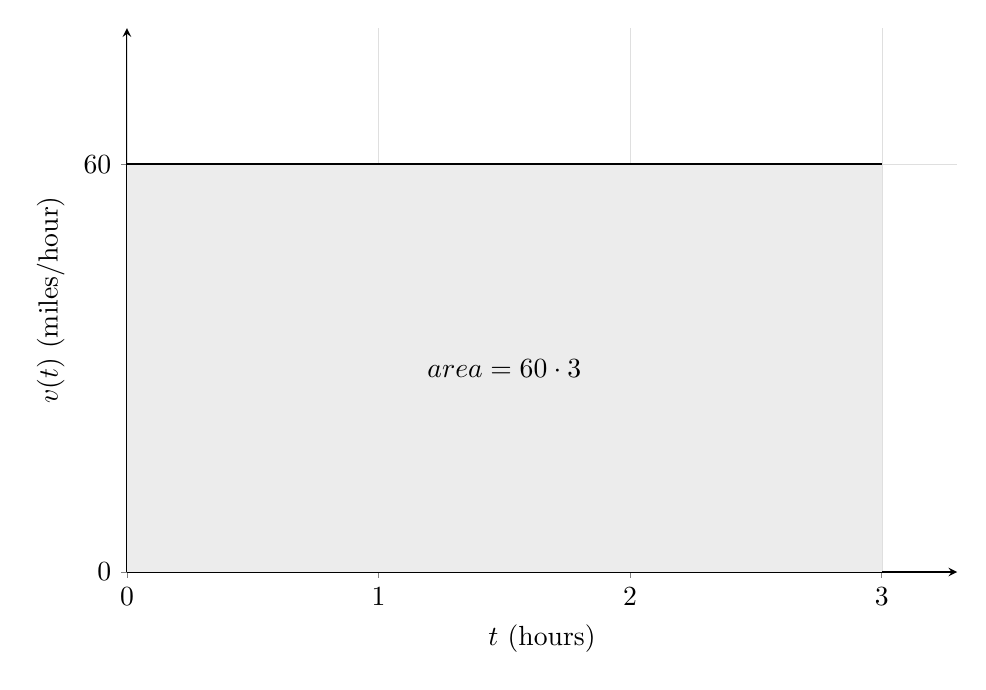
\begin{tikzpicture}
\begin{axis}[
    width=\textwidth,
    height=0.70\textwidth,
    xmin=0, xmax=3.3,
    ymin=0, ymax=80,
    axis lines=left,
    xlabel={\(t\) (hours)},
    ylabel={\(v(t)\) (miles/hour)},
    xtick={0,1,2,3},
    ytick={0,60},
    grid=both,
    grid style={line width=.1pt, draw=gray!25},
]
\draw[fill=gray!15,draw=none] (axis cs:0,0) rectangle (axis cs:3,60);
\addplot[thick,domain=0:3,samples=2] {60};
\node at (axis cs:1.5,30) {\(\text{area}=60\cdot 3\)};
\end{axis}
\end{tikzpicture}
\end{minipage}
\hfill
\begin{minipage}{0.47\textwidth}
\centering
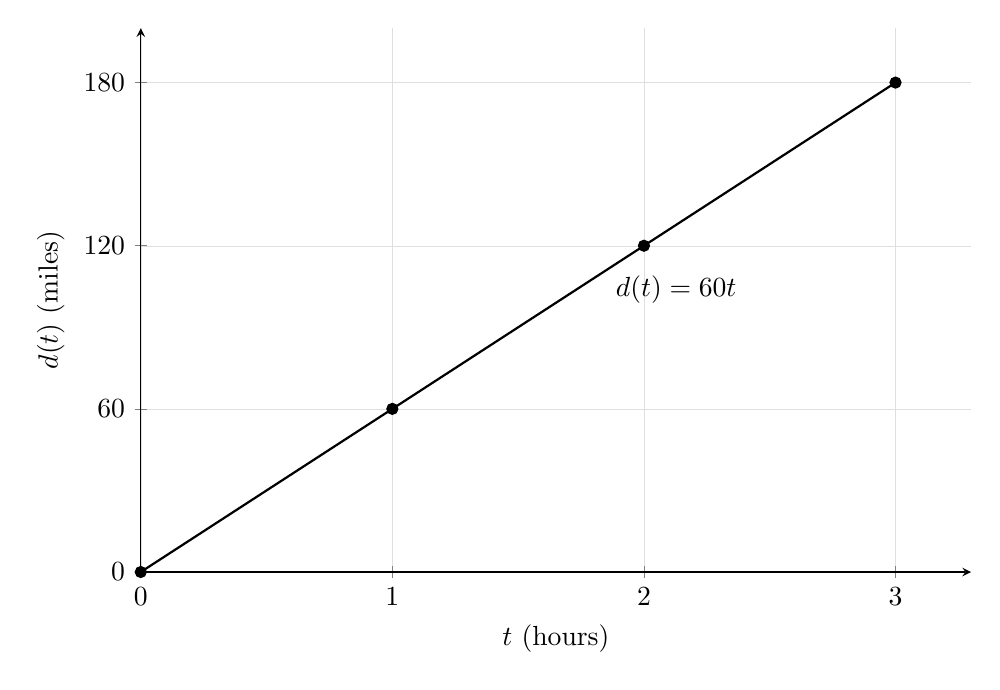
\begin{tikzpicture}
\begin{axis}[
    width=\textwidth,
    height=0.70\textwidth,
    xmin=0, xmax=3.3,
    ymin=0, ymax=200,
    axis lines=left,
    xlabel={\(t\) (hours)},
    ylabel={\(d(t)\) (miles)},
    xtick={0,1,2,3},
    ytick={0,60,120,180},
    grid=both,
    grid style={line width=.1pt, draw=gray!25},
]
\addplot[thick,domain=0:3,samples=2] {60*x};
\addplot[only marks,mark=*] coordinates {(0,0) (1,60) (2,120) (3,180)};
\node[anchor=west] at (axis cs:1.85,104) {\(d(t)=60t\)};
\end{axis}
\end{tikzpicture}
\end{minipage}
\caption{Constant velocity gives a horizontal velocity graph and a straight distance graph. The same number \(60\) appears as a height, a slope, and a rate.}
\label{fig:constant-velocity-graphs}
\end{figure}

The two graphs show the same trip in different languages.

On the velocity graph, \(60\) is a height.

On the distance graph, \(60\) is a slope.

\subsection{Slope of the distance graph}

Take two times \(a\) and \(b\), with \(a<b\). The average velocity from \(t=a\) to \(t=b\) is

\[
\frac{d(b)-d(a)}{b-a}.
\]

For \(d(t)=60t\),

\[
\frac{d(b)-d(a)}{b-a}
=
\frac{60b-60a}{b-a}
=
\frac{60(b-a)}{b-a}
=
60.
\]

The answer does not depend on which two times we choose. Every secant line has the same slope because the graph is already a straight line.

\begin{quote}
\textbf{Constant velocity appears as constant slope.}

If \(d(t)=60t\), then the slope of the distance graph is always \(60\), matching the velocity.
\end{quote}

More generally, if

\[
d(t)=d_0+v_0t,
\]

then

\[
\frac{d(b)-d(a)}{b-a}
=
v_0.
\]

The starting value \(d_0\) moves the line up or down, but it does not change the slope.

\paragraph{Example.}
Suppose

\[
d(t)=20+55t.
\]

Then \(d(0)=20\). The car has already accumulated \(20\) miles when we start watching. But the velocity is still \(55\) miles/hour because

\[
\frac{d(b)-d(a)}{b-a}
=
\frac{(20+55b)-(20+55a)}{b-a}
=
55.
\]

The constant \(20\) cancels. Slope measures change, not starting value.

\subsection{Area under the velocity graph}

Now start from the velocity graph instead. If

\[
v(t)=60
\]

from \(t=0\) to \(t=3\), then the region under the velocity graph is a rectangle.

Its height is \(60\) miles/hour. Its width is \(3\) hours. Its area is

\[
60\cdot 3=180.
\]

The units are

\[
\frac{\text{miles}}{\text{hour}}\cdot \text{hour}
=
\text{miles}.
\]

So the area under the velocity graph gives distance traveled:

\[
d(3)-d(0)=180.
\]

At a general time \(t\),

\[
\text{area under } v(t)=60 \text{ from }0\text{ to }t
=
60t.
\]

This is exactly the distance function

\[
d(t)=60t.
\]

\begin{quote}
\textbf{Constant velocity appears as rectangular area.}

If \(v(t)=60\), then the accumulated distance from \(0\) to \(t\) is the area of a rectangle:

\[
60t.
\]
\end{quote}

\subsection{The constant-velocity rule}

The same idea works on any time interval.

Suppose the velocity is constant:

\[
v(t)=v_0
\]

for \(a\leq t\leq b\). Then the distance traveled from time \(a\) to time \(b\) is

\[
v_0(b-a).
\]

Equivalently,

\[
\boxed{d(b)-d(a)=v_0(b-a).}
\]

This formula has two readings.

First, it is a slope statement:

\[
v_0=\frac{d(b)-d(a)}{b-a}.
\]

Second, it is an area statement:

\[
d(b)-d(a)=\text{area of a rectangle of height }v_0\text{ and width }b-a.
\]

The same rectangle that computes distance also explains why the distance graph has slope \(v_0\).

\subsection{Why slope and area are inverse clues}

For constant velocity, nothing mysterious is hidden.

Starting with distance,

\[
d(t)=d_0+v_0t,
\]

we find velocity by taking the slope:

\[
\frac{\text{change in distance}}{\text{change in time}}=v_0.
\]

Starting with velocity,

\[
v(t)=v_0,
\]

we find change in distance by taking rectangular area:

\[
\text{height}\cdot \text{width}=v_0(b-a).
\]

So the two dashboard questions become two geometric questions:

\[
\boxed{\text{velocity}=\text{slope of the distance graph}}
\]

and

\[
\boxed{\text{change in distance}=\text{area under the velocity graph}.}
\]

This is the first shape of calculus.

\subsection{Why the word ``constant'' matters}

The formula

\[
d(b)-d(a)=v_0(b-a)
\]

requires constant velocity. Without that assumption, it can give the wrong story.

Suppose a car travels

\[
30\text{ miles/hour for the first } \frac12\text{ hour}
\]

and then

\[
70\text{ miles/hour for the next } \frac12\text{ hour}.
\]

The total distance is

\[
30\cdot \frac12 +70\cdot \frac12
=
15+35
=
50
\]

miles.

The average velocity over the full hour is \(50\) miles/hour, but the car was never moving at \(50\) miles/hour during either half of the trip.

The velocity graph is no longer one horizontal line. It has two steps. The distance graph is no longer one straight line. It has two line segments, one with slope \(30\) and one with slope \(70\).

\begin{figure}[h]
\centering
\begin{minipage}{0.47\textwidth}
\centering
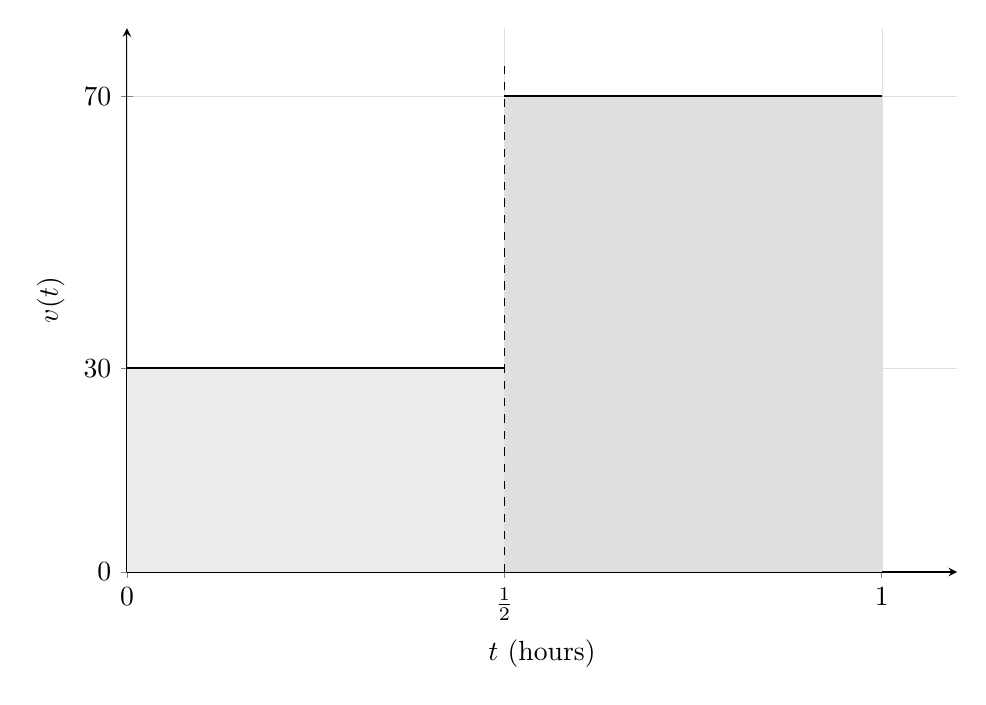
\begin{tikzpicture}
\begin{axis}[
    width=\textwidth,
    height=0.70\textwidth,
    xmin=0, xmax=1.1,
    ymin=0, ymax=80,
    axis lines=left,
    xlabel={\(t\) (hours)},
    ylabel={\(v(t)\)},
    xtick={0,0.5,1},
    xticklabels={\(0\),\(\frac12\),\(1\)},
    ytick={0,30,70},
    grid=both,
    grid style={line width=.1pt, draw=gray!25},
]
\draw[fill=gray!15,draw=none] (axis cs:0,0) rectangle (axis cs:0.5,30);
\draw[fill=gray!25,draw=none] (axis cs:0.5,0) rectangle (axis cs:1,70);
\addplot[thick] coordinates {(0,30) (0.5,30)};
\addplot[thick] coordinates {(0.5,70) (1,70)};
\draw[dashed] (axis cs:0.5,0) -- (axis cs:0.5,75);
\end{axis}
\end{tikzpicture}
\end{minipage}
\hfill
\begin{minipage}{0.47\textwidth}
\centering
\begin{tikzpicture}
\begin{axis}[
    width=\textwidth,
    height=0.70\textwidth,
    xmin=0, xmax=1.1,
    ymin=0, ymax=55,
    axis lines=left,
    xlabel={\(t\) (hours)},
    ylabel={\(d(t)\)},
    xtick={0,0.5,1},
    xticklabels={\(0\),\(\frac12\),\(1\)},
    ytick={0,15,50},
    grid=both,
    grid style={line width=.1pt, draw=gray!25},
]
\addplot[thick] coordinates {(0,0) (0.5,15) (1,50)};
\addplot[only marks,mark=*] coordinates {(0,0) (0.5,15) (1,50)};
\node[anchor=west] at (axis cs:0.1,14) {slope \(30\)};
\node[anchor=west] at (axis cs:0.52,41) {slope \(70\)};
\end{axis}
\end{tikzpicture}
\end{minipage}
\caption{When velocity changes by steps, distance is built from several straight pieces. Each piece has its own slope.}
\label{fig:piecewise-constant-preview}
\end{figure}

This example is still simple because the velocity is constant on each half-hour piece. We can add two rectangle areas.

But real motion rarely changes only once. A driver speeds up, slows down, stops, and starts again. The velocity graph may have many pieces, or no flat pieces at all.

The next step is to allow motion forward and backward. Then area below the time axis must count with a sign. That sign is not a technicality; it is how calculus remembers direction.
\section{Forward, backward, and signed motion}
\label{sec:signed-motion}

Constant velocity gave us the first picture of calculus: slope on one graph and area on another. But we quietly assumed that the car only moved forward. The moment a car can reverse, the dashboard story needs one more idea.

Velocity has a sign.

Choose one direction on a straight road and call it positive. For example, east may be positive and west negative. A car moving east at \(40\) miles/hour has velocity

\[
v=40.
\]

A car moving west at the same speed has velocity

\[
v=-40.
\]

The speed is the size of the velocity:

\[
\text{speed}=|v|.
\]

So speed is never negative, but velocity can be negative. This sign is how calculus remembers direction.

\subsection{Positive and negative velocity}

When motion can go backward, it is better to stop using \(d(t)\) for everything. The word ``distance'' usually means a nonnegative amount traveled. Instead, let

\[
s(t)
\]

denote the signed position of the car along the road at time \(t\). We measure \(s(t)\) in miles from the starting point, with positive values in the chosen positive direction.

If \(s(0)=0\), then:

\[
s(t)>0
\]

means the car is on the positive side of the starting point, while

\[
s(t)<0
\]

means the car is on the negative side.

The change

\[
s(b)-s(a)
\]

is called the \emph{displacement} from time \(a\) to time \(b\). Displacement is signed. It can be positive, negative, or zero.

\paragraph{Example.}
Suppose a car moves as follows:

\[
40\text{ miles/hour for }2\text{ hours},
\]

then

\[
-30\text{ miles/hour for }1\text{ hour}.
\]

The first part moves the car

\[
40\cdot 2=80
\]

miles in the positive direction. The second part moves the car

\[
-30\cdot 1=-30
\]

miles in the negative direction.

So the displacement over the whole trip is

\[
80+(-30)=50
\]

miles.

The car ends \(50\) miles ahead of where it started.

\subsection{Displacement versus distance traveled}

The odometer would tell a different story. The car actually drove \(80\) miles forward and then \(30\) miles backward. The total distance traveled is

\[
80+30=110
\]

miles.

So in this trip,

\[
\text{displacement}=50\text{ miles},
\]

but

\[
\text{distance traveled}=110\text{ miles}.
\]

These are not the same.

\begin{quote}
\textbf{Displacement remembers direction.}

Forward motion counts positive. Backward motion counts negative.

\[
\text{displacement}=s(b)-s(a).
\]

\textbf{Distance traveled ignores direction.}

Forward and backward motion both add positive length.

\[
\text{distance traveled}=\text{sum of the lengths of all pieces of motion}.
\]
\end{quote}

A person who walks \(10\) steps forward and \(10\) steps backward has displacement \(0\), but did not stand still. The distance traveled is \(20\) steps.

\subsection{Area below the time axis}

Now look at the velocity graph. Positive velocity lies above the time axis. Negative velocity lies below it.

For the trip above,

\[
v(t)=
\begin{cases}
40, & 0\leq t<2,\\
-30, & 2<t\leq 3.
\end{cases}
\]

The signed position is

\[
s(t)=
\begin{cases}
40t, & 0\leq t\leq 2,\\
80-30(t-2), & 2\leq t\leq 3.
\end{cases}
\]

At \(t=2\), the simple model changes velocity instantly. We may leave \(v(2)\) undefined. That one instant has no width, so it does not affect any accumulated displacement in this step model. But it does leave a corner in the graph of \(s(t)\). Later, that corner will matter when we ask for instantaneous velocity.

\begin{figure}[h]
\centering
\begin{minipage}{0.47\textwidth}
\centering
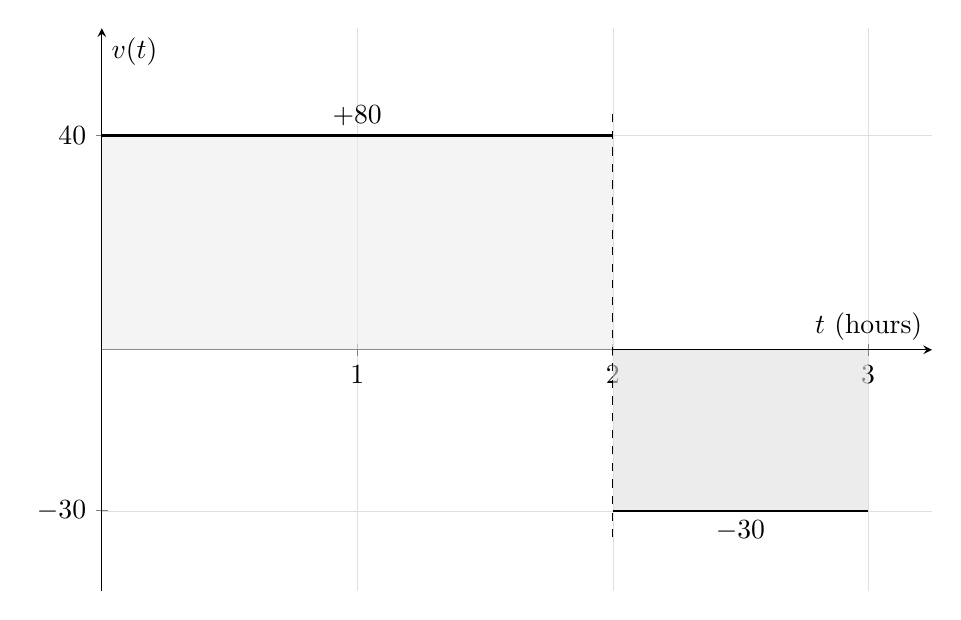
\begin{tikzpicture}
\begin{axis}[
    width=\textwidth,
    height=0.72\textwidth,
    xmin=0, xmax=3.25,
    ymin=-45, ymax=60,
    axis lines=middle,
    xlabel={\(t\) (hours)},
    ylabel={\(v(t)\)},
    xtick={0,1,2,3},
    ytick={-30,0,40},
    grid=both,
    grid style={line width=.1pt, draw=gray!25},
]
\draw[fill=gray!15, fill opacity=0.6, draw=none] (axis cs:0,0) rectangle (axis cs:2,40);
\draw[fill=gray!25, fill opacity=0.6, draw=none] (axis cs:2,0) rectangle (axis cs:3,-30);
\addplot[thick] coordinates {(0,40) (2,40)};
\addplot[thick] coordinates {(2,-30) (3,-30)};
\draw[dashed] (axis cs:2,-35) -- (axis cs:2,45);
\node[anchor=south] at (axis cs:1,40) {\(+80\)};
\node[anchor=north] at (axis cs:2.5,-30) {\(-30\)};
\end{axis}
\end{tikzpicture}
\end{minipage}
\hfill
\begin{minipage}{0.47\textwidth}
\centering
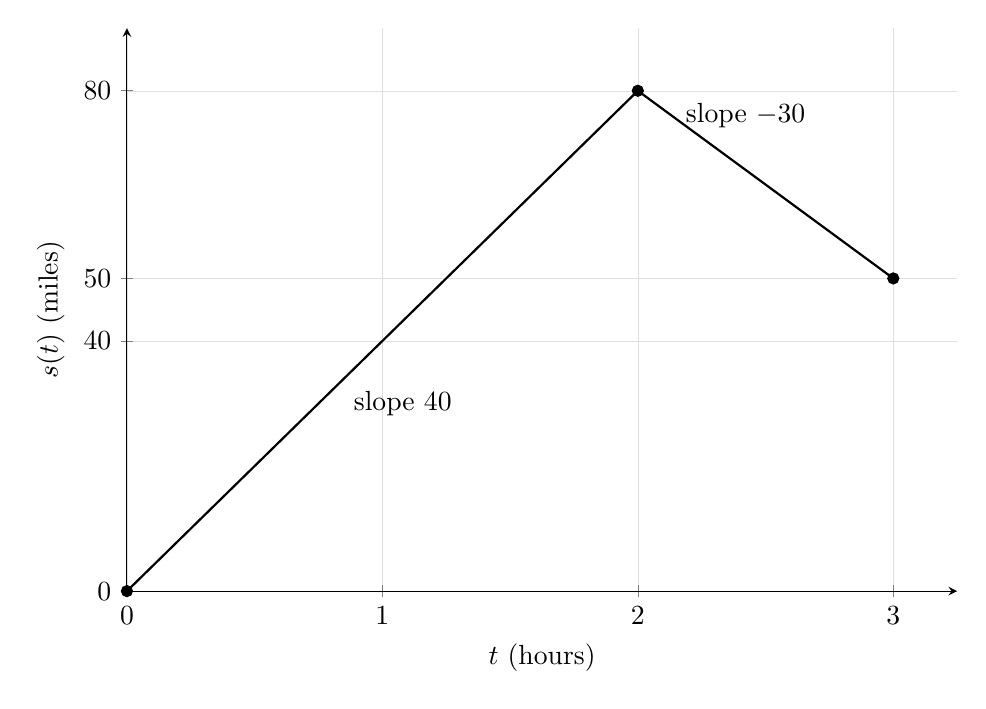
\begin{tikzpicture}
\begin{axis}[
    width=\textwidth,
    height=0.72\textwidth,
    xmin=0, xmax=3.25,
    ymin=0, ymax=90,
    axis lines=left,
    xlabel={\(t\) (hours)},
    ylabel={\(s(t)\) (miles)},
    xtick={0,1,2,3},
    ytick={0,40,50,80},
    grid=both,
    grid style={line width=.1pt, draw=gray!25},
]
\addplot[thick] coordinates {(0,0) (2,80) (3,50)};
\addplot[only marks,mark=*] coordinates {(0,0) (2,80) (3,50)};
\node[anchor=west] at (axis cs:0.85,30) {slope \(40\)};
\node[anchor=west] at (axis cs:2.15,76) {slope \(-30\)};
\end{axis}
\end{tikzpicture}
\end{minipage}
\caption{Area above the time axis counts positive. Area below the time axis counts negative. The signed area under the velocity graph is \(80-30=50\), matching the change in signed position.}
\label{fig:signed-area-motion}
\end{figure}

The area above the time axis is a rectangle of height \(40\) and width \(2\):

\[
40\cdot 2=80.
\]

The area below the time axis is a rectangle of height \(30\) and width \(1\), but it counts negatively:

\[
-30\cdot 1=-30.
\]

Therefore the signed area under the velocity graph is

\[
80-30=50.
\]

This equals

\[
s(3)-s(0)=50-0=50.
\]

So the rule from constant velocity survives, but with a sign:

\[
\boxed{\text{change in signed position}=\text{signed area under the velocity graph}.}
\]

\subsection{A first piecewise-defined motion}

A formula such as

\[
v(t)=
\begin{cases}
40, & 0\leq t<2,\\
-30, & 2<t\leq 3
\end{cases}
\]

is called \emph{piecewise-defined}. It gives different instructions on different pieces of the domain.

Piecewise-defined functions are not artificial. They describe many real situations:

\[
\begin{array}{c|c}
\text{motion} & \text{piecewise behavior} \\ \hline
\text{a car stops at a red light} & \text{positive velocity, then zero velocity} \\
\text{an elevator goes up, stops, then goes down} & \text{positive, zero, negative velocity} \\
\text{a thermostat turns heat on and off} & \text{different rules at different temperatures} \\
\text{a tax bracket changes} & \text{different rates on different income intervals}
\end{array}
\]

In a piecewise-constant velocity model, each time interval is easy. The velocity is constant on that interval, so displacement is

\[
\text{velocity}\cdot \text{time}.
\]

Then we add the pieces.

\paragraph{Example.}
Suppose a car has velocity

\[
v(t)=
\begin{cases}
50, & 0\leq t<1,\\
0, & 1\leq t<2,\\
-20, & 2\leq t\leq 4.
\end{cases}
\]

The displacement from \(0\) to \(4\) is

\[
50\cdot 1+0\cdot 1+(-20)\cdot 2
=
50+0-40
=
10.
\]

The car ends \(10\) miles ahead of where it started.

The distance traveled is

\[
|50|\cdot 1+|0|\cdot 1+|-20|\cdot 2
=
50+0+40
=
90.
\]

The signed calculation tells where the car ends. The absolute-value calculation tells how much road the car has covered.

\subsection{What the sign prepares us for}

Signed area is not ordinary geometric area. Ordinary geometric area is never negative. Signed area is different because it is designed to represent accumulated change.

If \(v(t)>0\), the signed position increases.

If \(v(t)<0\), the signed position decreases.

If \(v(t)=0\), the signed position does not change.

That is why the graph of \(s(t)\) rises, falls, or stays flat according to the sign of \(v(t)\).

For piecewise-constant velocity, we can compute everything with rectangles. But the next idea is even simpler and deeper: if we know a list of signed positions at equally spaced times, then the changes between them contain all the information needed to recover the final position from the first one.

That is calculus before limits.

\section{Calculus without limits: finite differences and finite sums}
\label{sec:calculus-without-limits}

Signed motion taught us to add changes with their signs. Now we strip the story down to its arithmetic core.

Suppose we record the signed position of a car at whole-number times:

\[
\begin{array}{c|rrrrrr}
j & 0 & 1 & 2 & 3 & 4 & 5 \\ \hline
s_j & 0 & 2 & 6 & 7 & 4 & 9
\end{array}
\]

Here \(s_j\) means the signed position at time \(j\). The car starts at \(0\), moves to \(2\), then to \(6\), then to \(7\), then back to \(4\), then forward to \(9\).

The changes between consecutive positions are

\[
\begin{array}{c|rrrrr}
j & 1 & 2 & 3 & 4 & 5 \\ \hline
\Delta s_j & 2 & 4 & 1 & -3 & 5
\end{array}
\]

The symbol \(\Delta\) means ``change in.'' Thus

\[
\Delta s_j=s_j-s_{j-1}.
\]

For example,

\[
\Delta s_4=s_4-s_3=4-7=-3.
\]

That negative value says the car moved backward during the fourth interval.

\subsection{Difference tables}

A table of values produces a table of differences:

\[
\begin{array}{c|rrrrrr}
j & 0 & 1 & 2 & 3 & 4 & 5 \\ \hline
s_j & 0 & 2 & 6 & 7 & 4 & 9 \\
\Delta s_j & & 2 & 4 & 1 & -3 & 5
\end{array}
\]

If each time interval has length \(1\), then the numerical values of the differences are also the average velocities on those intervals:

\[
\text{average velocity on interval }j
=
\frac{s_j-s_{j-1}}{1}
=
\Delta s_j.
\]

The units still matter. If \(s\) is measured in miles and time is measured in hours, then \(\Delta s_j\) is measured in miles, while

\[
\frac{\Delta s_j}{1}
\]

is measured in miles/hour. The numbers match only because the time step is \(1\).

\subsection{Accumulated differences telescope}

Now add all the changes:

\[
2+4+1-3+5=9.
\]

This equals the final position minus the initial position:

\[
s_5-s_0=9-0=9.
\]

That is not an accident. Watch the cancellation:

\[
\begin{aligned}
\Delta s_1+\Delta s_2+\Delta s_3+\Delta s_4+\Delta s_5
&=(s_1-s_0)+(s_2-s_1)+(s_3-s_2)+(s_4-s_3)+(s_5-s_4)\\
&=s_5-s_0.
\end{aligned}
\]

Every inside value appears once with a plus sign and once with a minus sign. Only the final value and the initial value remain.

This kind of cancellation is called \emph{telescoping}. A long sum collapses, the way a telescope collapses into a shorter tube.

For any finite list

\[
s_0,s_1,s_2,\ldots,s_n,
\]

we have

\[
\boxed{\Delta s_1+\Delta s_2+\cdots+\Delta s_n=s_n-s_0.}
\]

Using summation notation, this is

\[
\boxed{\sum_{j=1}^{n}\Delta s_j=s_n-s_0.}
\]

The symbol \(\sum\) means ``add.'' So

\[
\sum_{j=1}^{n}\Delta s_j
\]

means

\[
\Delta s_1+\Delta s_2+\cdots+\Delta s_n.
\]

\subsection{Step velocities and piecewise linear position}

Now give the same arithmetic a graph.

Suppose the velocity is constant on each interval of length \(1\):

\[
v_1=2,\qquad v_2=4,\qquad v_3=1,\qquad v_4=-3,\qquad v_5=5.
\]

Starting from \(s_0=0\), the positions become

\[
s_1=2,\qquad
s_2=6,\qquad
s_3=7,\qquad
s_4=4,\qquad
s_5=9.
\]

The velocity graph is made of flat steps. The position graph is made of straight line segments.

\begin{figure}[h]
\centering
\begin{minipage}{0.47\textwidth}
\centering
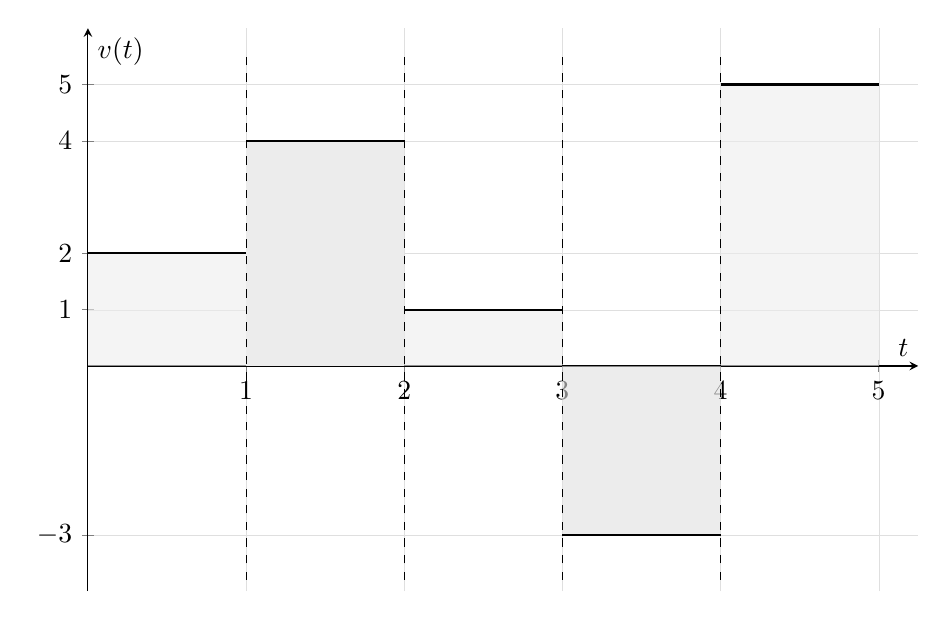
\begin{tikzpicture}
\begin{axis}[
    width=\textwidth,
    height=0.72\textwidth,
    xmin=0, xmax=5.25,
    ymin=-4, ymax=6,
    axis lines=middle,
    xlabel={\(t\)},
    ylabel={\(v(t)\)},
    xtick={0,1,2,3,4,5},
    ytick={-3,0,1,2,4,5},
    grid=both,
    grid style={line width=.1pt, draw=gray!25},
]
\draw[fill=gray!15,fill opacity=0.6, draw=none]  (axis cs:0,0) rectangle (axis cs:1,2);
\draw[fill=gray!15,draw=none] (axis cs:1,0) rectangle (axis cs:2,4);
\draw[fill=gray!15,fill opacity=0.6,draw=none] (axis cs:2,0) rectangle (axis cs:3,1);
\draw[fill=gray!25,fill opacity=0.6,draw=none] (axis cs:3,0) rectangle (axis cs:4,-3);
\draw[fill=gray!15,fill opacity=0.6,draw=none] (axis cs:4,0) rectangle (axis cs:5,5);

\addplot[thick] coordinates {(0,2) (1,2)};
\addplot[thick] coordinates {(1,4) (2,4)};
\addplot[thick] coordinates {(2,1) (3,1)};
\addplot[thick] coordinates {(3,-3) (4,-3)};
\addplot[thick] coordinates {(4,5) (5,5)};

\pgfplotsinvokeforeach{1,2,3,4}{
  \draw[dashed] (axis cs:#1,-3.8) -- (axis cs:#1,5.6);
}
\end{axis}
\end{tikzpicture}
\end{minipage}
\hfill
\begin{minipage}{0.47\textwidth}
\centering
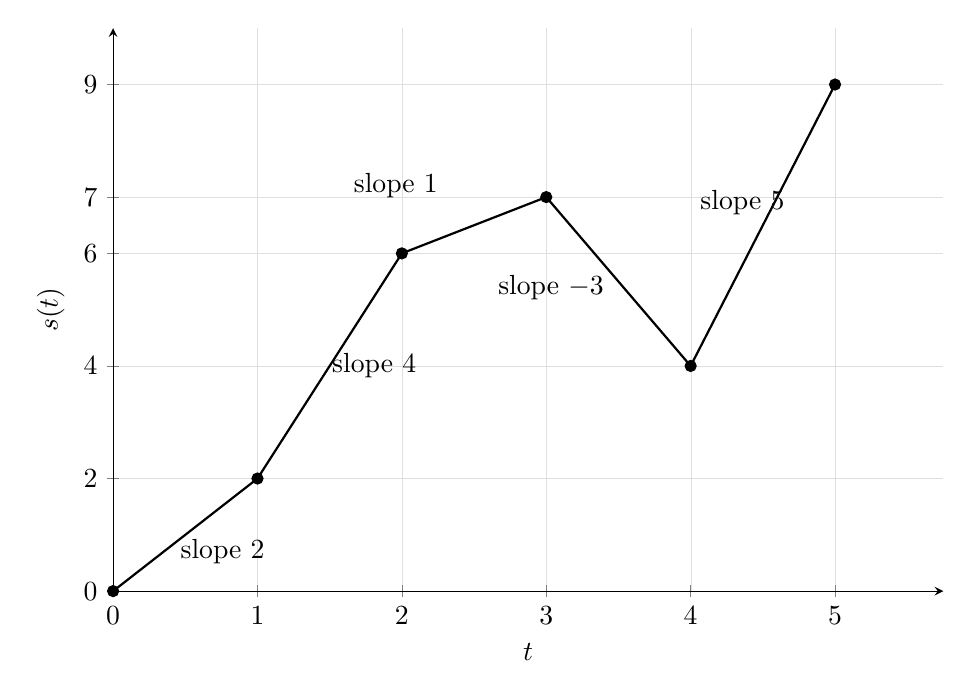
\begin{tikzpicture}
\begin{axis}[
    width=\textwidth,
    height=0.72\textwidth,
    xmin=0, xmax=5.75,
    ymin=0, ymax=10,
    axis lines=left,
    xlabel={\(t\)},
    ylabel={\(s(t)\)},
    xtick={0,1,2,3,4,5},
    ytick={0,2,4,6,7,9},
    grid=both,
    grid style={line width=.1pt, draw=gray!25},
]
\addplot[thick] coordinates {(0,0) (1,2) (2,6) (3,7) (4,4) (5,9)};
\addplot[only marks,mark=*] coordinates {(0,0) (1,2) (2,6) (3,7) (4,4) (5,9)};
\node[anchor=west] at (axis cs:0.4,0.7) {slope \(2\)};
\node[anchor=west] at (axis cs:1.45,4.0) {slope \(4\)};
\node[anchor=west] at (axis cs:1.6,7.2) {slope \(1\)};
\node[anchor=west] at (axis cs:2.6,5.4) {slope \(-3\)};
\node[anchor=west] at (axis cs:4.0,6.9) {slope \(5\)};
\end{axis}
\end{tikzpicture}
\end{minipage}
\caption{Step velocity gives a piecewise linear position graph. The signed rectangle areas \(2+4+1-3+5\) equal the net change \(9-0\).}
\label{fig:finite-ftc-step-velocity}
\end{figure}

On each interval, the slope of the position graph is the velocity on that interval.

The signed area under the velocity graph is

\[
2\cdot 1+4\cdot 1+1\cdot 1+(-3)\cdot 1+5\cdot 1=9.
\]

The change in position is

\[
s(5)-s(0)=9-0=9.
\]

So the picture says exactly what the arithmetic said.

\subsection{Unequal time steps}

The time intervals do not need to have length \(1\). Suppose

\[
t_0<t_1<t_2<\cdots<t_n
\]

and the \(j\)-th time interval has width

\[
\Delta t_j=t_j-t_{j-1}.
\]

If the velocity is constant and equal to \(v_j\) on that interval, then

\[
s_j-s_{j-1}=v_j\Delta t_j.
\]

Adding all intervals gives

\[
(s_1-s_0)+(s_2-s_1)+\cdots+(s_n-s_{n-1})
=
v_1\Delta t_1+v_2\Delta t_2+\cdots+v_n\Delta t_n.
\]

The left side telescopes to \(s_n-s_0\). Therefore

\[
\boxed{s_n-s_0=\sum_{j=1}^{n} v_j\Delta t_j.}
\]

Each product

\[
v_j\Delta t_j
\]

is the signed area of one rectangle in the velocity graph.

\begin{quote}
\textbf{Finite version of the Fundamental Theorem.}

For step velocity and piecewise linear position,

\[
\boxed{\text{signed area under velocity}=\text{change in position}.}
\]

Equivalently,

\[
\boxed{\sum_{j=1}^{n} v_j\Delta t_j=s_n-s_0.}
\]
\end{quote}

This is not yet the full Fundamental Theorem of Calculus. It is its finite ancestor. No limits are needed because every velocity graph here is made of finitely many flat pieces.

\subsection{A warning about absolute values}

The telescoping rule works for signed changes:

\[
\sum_{j=1}^{n}\Delta s_j=s_n-s_0.
\]

It does not work for total distance traveled.

For the table

\[
\begin{array}{c|rrrrrr}
j & 0 & 1 & 2 & 3 & 4 & 5 \\ \hline
s_j & 0 & 2 & 6 & 7 & 4 & 9 \\
\Delta s_j & & 2 & 4 & 1 & -3 & 5
\end{array}
\]

the displacement is

\[
2+4+1-3+5=9.
\]

The distance traveled is

\[
|2|+|4|+|1|+|-3|+|5|
=
2+4+1+3+5
=
15.
\]

The negative step cancels in displacement, but it adds to distance traveled. This is why the sign of velocity matters.

\subsection{Squares and odd numbers}

Finite differences reveal patterns that are easy to miss in the original values.

Consider the square numbers:

\[
0,\ 1,\ 4,\ 9,\ 16,\ 25,\ldots
\]

These are

\[
s_j=j^2.
\]

The differences are

\[
\Delta s_j=s_j-s_{j-1}=j^2-(j-1)^2.
\]

Compute:

\[
j^2-(j-1)^2
=
j^2-(j^2-2j+1)
=
2j-1.
\]

So the differences of the square numbers are the odd numbers:

\[
1,\ 3,\ 5,\ 7,\ 9,\ldots
\]

Now telescope:

\[
\sum_{j=1}^{n}(2j-1)
=
\sum_{j=1}^{n}\bigl(j^2-(j-1)^2\bigr)
=
n^2-0^2.
\]

Therefore

\[
\boxed{1+3+5+\cdots+(2n-1)=n^2.}
\]

This is a small but beautiful example of the same idea. Differences undo sums. Sums undo differences.

\subsection{What finite calculus can and cannot do}

Finite differences answer one question:

\[
\text{Given positions }s_0,s_1,\ldots,s_n,\text{ find the step velocities.}
\]

Finite sums answer the reverse question:

\[
\text{Given step velocities }v_1,\ldots,v_n,\text{ recover the change in position.}
\]

So even before limits, we see the two directions of calculus:

\[
\text{position}\longrightarrow \text{change}
\]

and

\[
\text{change}\longrightarrow \text{position}.
\]

But real motion is usually not made of perfect steps. A car does not hold one exact velocity for a while, jump instantly to another, and hold that forever. Its velocity changes while the clock is running.

For a changing velocity, rectangles are no longer exact. They become estimates. The natural response is to use shorter intervals, then shorter ones still.

That is where limits enter.
\section{Changing velocity and the need for limits}
\label{sec:changing-velocity-limits}

Step velocities were friendly. On each interval, the velocity graph was flat, so a rectangle gave exact displacement and a line segment gave exact position.

Real motion is not usually so polite. A car speeds up while the clock is running. A falling stone moves faster at each instant. A population grows at a rate that changes with its size. The old rectangle and slope pictures still guide us, but now they are no longer exact after only finitely many pieces.

The new idea is to look closer and closer.

\subsection{Average velocity over a time interval}

Let \(s(t)\) be signed position at time \(t\). If \(a\neq b\), the average velocity from time \(a\) to time \(b\) is

\[
\overline v_{[a,b]}
=
\frac{s(b)-s(a)}{b-a}.
\]

This is the same formula we have used since the dashboard:

\[
\frac{\text{change in position}}{\text{change in time}}.
\]

The denominator cannot be zero. Average velocity needs an interval of time, not a single instant.

\paragraph{Example.}
Suppose a toy motion has signed position

\[
s(t)=t^2.
\]

The formula is chosen because the arithmetic is simple. The average velocity from \(t=2\) to \(t=3\) is

\[
\frac{s(3)-s(2)}{3-2}
=
\frac{9-4}{1}
=
5.
\]

The average velocity from \(t=2\) to \(t=2.1\) is

\[
\frac{s(2.1)-s(2)}{2.1-2}
=
\frac{4.41-4}{0.1}
=
4.1.
\]

The shorter interval gives a number closer to what we expect the velocity to be at the instant \(t=2\).

To see the pattern, write the nearby time as \(2+h\). Then

\[
\frac{s(2+h)-s(2)}{h}
=
\frac{(2+h)^2-2^2}{h}.
\]

Expanding the numerator,

\[
(2+h)^2-2^2
=
4+4h+h^2-4
=
4h+h^2.
\]

So for \(h\neq 0\),

\[
\frac{s(2+h)-s(2)}{h}
=
\frac{4h+h^2}{h}
=
4+h.
\]

The number \(h\) is the time step. It may be positive or negative, but it cannot equal \(0\) inside this fraction.

\[
\begin{array}{c|rrrrrr}
h & 1 & 0.5 & 0.1 & 0.01 & -0.1 & -0.01 \\ \hline
\dfrac{s(2+h)-s(2)}{h}
& 5 & 4.5 & 4.1 & 4.01 & 3.9 & 3.99
\end{array}
\]

As \(h\) gets closer to \(0\), the average velocities get closer to \(4\). So the instantaneous velocity at \(t=2\) should be

\[
4.
\]

We have just used the idea of a limit. We have not yet defined limits carefully, but the picture is already clear:

\[
\boxed{
\text{instantaneous velocity}
=
\text{the value approached by average velocities over shrinking intervals.}
}
\]

For this example,

\[
v(2)=\lim_{h\to 0}\frac{s(2+h)-s(2)}{h}=4.
\]

The notation \(\lim_{h\to 0}\) means that \(h\) is allowed to get closer and closer to \(0\), while \(h\) itself remains nonzero during the calculation.

\subsection{The word ``if'' matters}

The average velocities must approach a single number. That does not always happen.

Recall the forward-then-backward motion from Section~\ref{sec:signed-motion}. In one simplified model,

\[
s(t)=
\begin{cases}
40t, & 0\leq t\leq 2,\\
80-30(t-2), & 2\leq t\leq 3.
\end{cases}
\]

Before \(t=2\), the slope is \(40\). After \(t=2\), the slope is \(-30\). The graph has a corner at \(t=2\).

If we approach \(t=2\) from the left, the average velocities approach \(40\). If we approach from the right, they approach \(-30\). There is no single velocity at the switching instant in this idealized model.

\begin{quote}
A derivative is born only when the nearby average rates settle toward one value.
\end{quote}

This is why calculus needs limits. The phrase ``gets close to'' must become precise enough to decide whether one number is really being approached.

\subsection{The tangent line problem}

Average velocity has a geometric twin: secant slope.

For a graph \(y=s(t)\), the average velocity from \(t=a\) to \(t=a+h\) is

\[
\frac{s(a+h)-s(a)}{h}.
\]

This is the slope of the secant line through the two points

\[
(a,s(a))
\quad\text{and}\quad
(a+h,s(a+h)).
\]

If these secant slopes approach one number as \(h\to0\), the limiting line is called the tangent line.

For \(s(t)=t^2\) at \(t=2\), the limiting slope is \(4\). The tangent line passes through \((2,4)\), so its equation is

\[
y-4=4(t-2).
\]

Equivalently,

\[
y=4t-4.
\]

\begin{figure}[h]
\centering
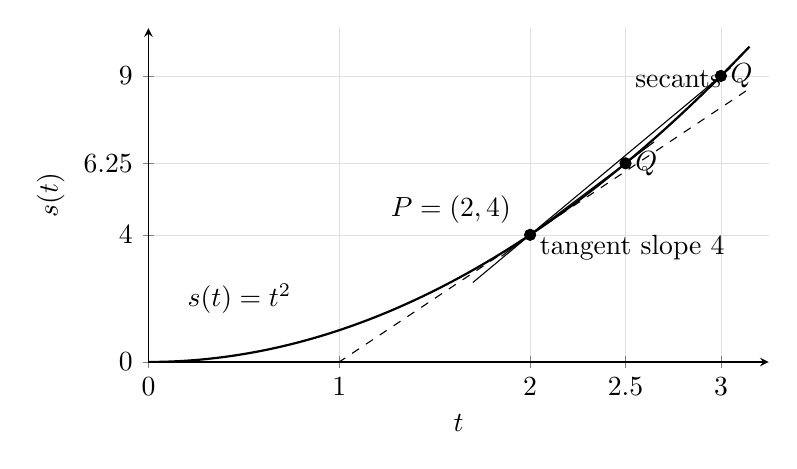
\begin{tikzpicture}
\begin{axis}[
    width=0.78\textwidth,
    height=0.48\textwidth,
    xmin=0, xmax=3.25,
    ymin=0, ymax=10.5,
    axis lines=left,
    xlabel={\(t\)},
    ylabel={\(s(t)\)},
    xtick={0,1,2,2.5,3},
    ytick={0,4,6.25,9},
    grid=both,
    grid style={line width=.1pt, draw=gray!25},
]
\addplot[thick,domain=0:3.15,samples=100] {x^2};
\addplot[domain=0.85:3.15,samples=2,dashed] {4*x-4};
\addplot[domain=1.7:3.05,samples=2] {5*x-6};
\addplot[domain=1.85:2.65,samples=2] {4.5*x-5};

\addplot[only marks,mark=*] coordinates {(2,4)};
\addplot[only marks,mark=*] coordinates {(3,9) (2.5,6.25)};

\node[anchor=south east] at (axis cs:1.95,4.05) {\(P=(2,4)\)};
\node[anchor=west] at (axis cs:3,9) {\(Q\)};
\node[anchor=west] at (axis cs:2.5,6.25) {\(Q\)};
\node[anchor=west] at (axis cs:2.5,8.9) {secants};
\node[anchor=west] at (axis cs:2.0,3.6) {tangent slope \(4\)};
\node[anchor=east] at (axis cs:0.8,2.0) {\(s(t)=t^2\)};
\end{axis}
\end{tikzpicture}
\caption{As the second point \(Q\) moves toward \(P\), the secant lines approach the tangent line. The slope of that tangent line is the instantaneous velocity.}
\label{fig:secants-to-tangent}
\end{figure}

At this stage, the tangent line is not merely a line that touches the curve. Some tangent lines cross the curve. Some lines can touch a graph without being the right tangent. The tangent line is the line obtained from limiting secant lines.

This changes the question from geometry to arithmetic:

\[
\boxed{
\text{Find the tangent slope}
\quad
\Longleftrightarrow
\quad
\text{find a limit of average rates.}
}
\]

\subsection{The area problem}

Now reverse the story. Suppose we know velocity and want displacement.

If the velocity is constant on each time interval, rectangles give the exact answer. But suppose the velocity changes continuously, for example

\[
v(t)=t^2
\]

from \(t=0\) to \(t=2\).

The graph is curved. No finite collection of rectangles naturally gives the exact area under it. But rectangles can estimate the area.

Divide the interval \([0,2]\) into \(n\) equal parts. Each part has width

\[
\Delta t=\frac{2}{n}.
\]

For \(n=4\), the width is \(\Delta t=\frac12\).

Using left endpoints gives a lower estimate, because \(t^2\) is increasing:

\[
L_4
=
\frac12\left(0^2+\left(\frac12\right)^2+1^2+\left(\frac32\right)^2\right)
=
\frac12\left(0+\frac14+1+\frac94\right)
=
\frac74
=
1.75.
\]

Using right endpoints gives an upper estimate:

\[
R_4
=
\frac12\left(\left(\frac12\right)^2+1^2+\left(\frac32\right)^2+2^2\right)
=
\frac12\left(\frac14+1+\frac94+4\right)
=
\frac{15}{4}
=
3.75.
\]

So the true area is somewhere between \(1.75\) and \(3.75\). That is a large window, but it is a start.

\begin{figure}[h]
\centering
\begin{minipage}{0.47\textwidth}
\centering
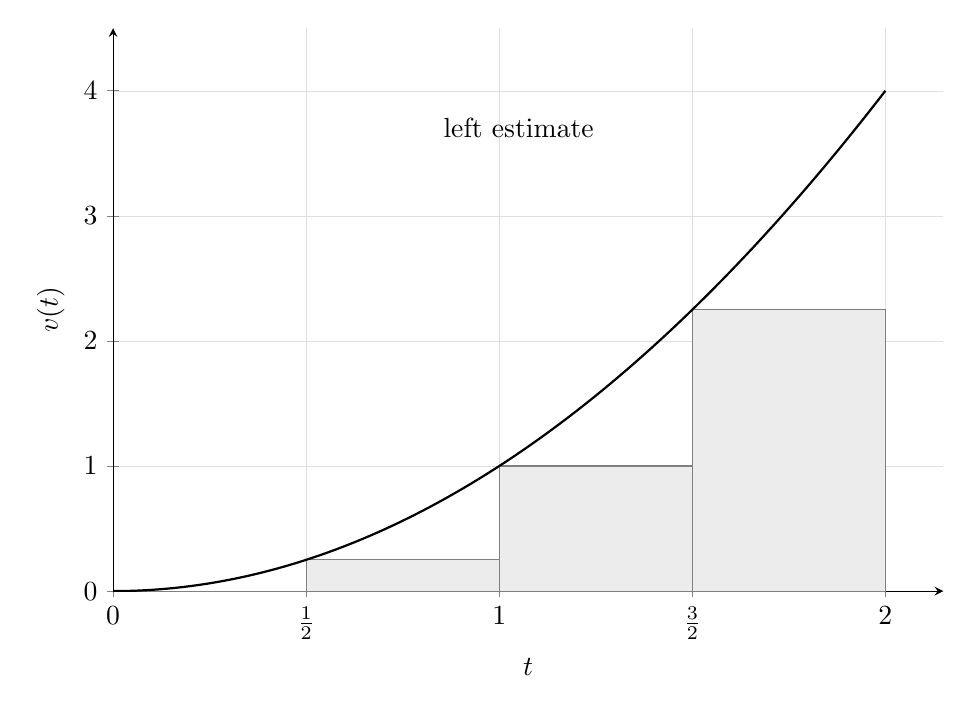
\begin{tikzpicture}
\begin{axis}[
    width=\textwidth,
    height=0.72\textwidth,
    xmin=0, xmax=2.15,
    ymin=0, ymax=4.5,
    axis lines=left,
    xlabel={\(t\)},
    ylabel={\(v(t)\)},
    xtick={0,0.5,1,1.5,2},
    xticklabels={\(0\),\(\frac12\),\(1\),\(\frac32\),\(2\)},
    ytick={0,1,2,3,4},
    grid=both,
    grid style={line width=.1pt, draw=gray!25},
]
\draw[fill=gray!15,draw=gray] (axis cs:0,0) rectangle (axis cs:0.5,0);
\draw[fill=gray!15,draw=gray] (axis cs:0.5,0) rectangle (axis cs:1,0.25);
\draw[fill=gray!15,draw=gray] (axis cs:1,0) rectangle (axis cs:1.5,1);
\draw[fill=gray!15,draw=gray] (axis cs:1.5,0) rectangle (axis cs:2,2.25);
\addplot[thick,domain=0:2,samples=100] {x^2};
\node at (axis cs:1.05,3.7) {left estimate};
\end{axis}
\end{tikzpicture}
\end{minipage}
\hfill
\begin{minipage}{0.47\textwidth}
\centering
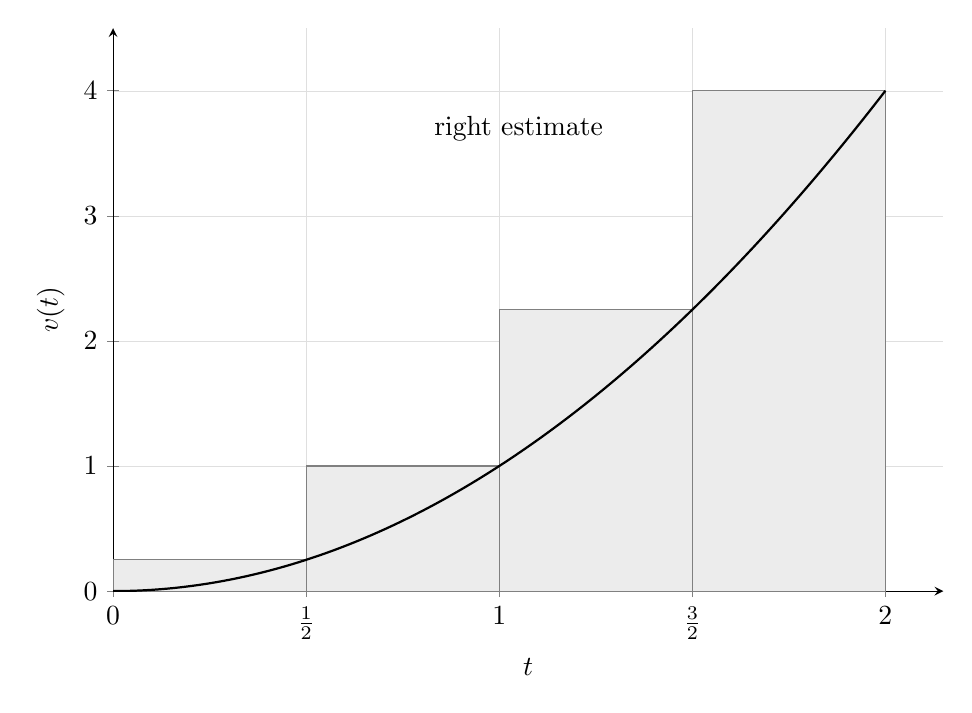
\begin{tikzpicture}
\begin{axis}[
    width=\textwidth,
    height=0.72\textwidth,
    xmin=0, xmax=2.15,
    ymin=0, ymax=4.5,
    axis lines=left,
    xlabel={\(t\)},
    ylabel={\(v(t)\)},
    xtick={0,0.5,1,1.5,2},
    xticklabels={\(0\),\(\frac12\),\(1\),\(\frac32\),\(2\)},
    ytick={0,1,2,3,4},
    grid=both,
    grid style={line width=.1pt, draw=gray!25},
]
\draw[fill=gray!15,draw=gray] (axis cs:0,0) rectangle (axis cs:0.5,0.25);
\draw[fill=gray!15,draw=gray] (axis cs:0.5,0) rectangle (axis cs:1,1);
\draw[fill=gray!15,draw=gray] (axis cs:1,0) rectangle (axis cs:1.5,2.25);
\draw[fill=gray!15,draw=gray] (axis cs:1.5,0) rectangle (axis cs:2,4);
\addplot[thick,domain=0:2,samples=100] {x^2};
\node at (axis cs:1.05,3.7) {right estimate};
\end{axis}
\end{tikzpicture}
\end{minipage}
\caption{For an increasing velocity \(v(t)=t^2\), left rectangles underestimate the area and right rectangles overestimate it. More rectangles make both estimates better.}
\label{fig:left-right-area-estimates}
\end{figure}

Using more rectangles improves the estimates.

\[
\begin{array}{c|ccc}
n & L_n & M_n & R_n \\ \hline
4  & 1.7500 & 2.6250 & 3.7500\\
8  & 2.1875 & 2.65625 & 3.1875\\
16 & 2.421875 & 2.6640625 & 2.921875
\end{array}
\]

Here \(M_n\) is the midpoint estimate, which uses the height of the curve at the middle of each subinterval.

The left and right estimates squeeze closer together. The midpoint estimate settles even faster. The number they approach is the area under the curve. Later we will call it

\[
\int_0^2 t^2\,dt.
\]

The exact value will turn out to be

\(
\frac83.
\)

For now, the important point is not the answer. It is the method:

\[
\boxed{
\text{area under a changing graph}
=
\text{the value approached by better and better rectangle sums.}
}
\]

\subsection{Why finite arithmetic is no longer enough}

Finite differences and finite sums worked perfectly for step motion.

If velocity is constant on each of finitely many intervals, then displacement is exactly

\[
\sum_{j=1}^{n} v_j\Delta t_j.
\]

But if velocity changes at every instant, no finite list of rectangles can fully capture the graph. We need an idea that lets infinitely many improving finite estimates settle toward one number.

That idea is a limit.

Limits will let us define:

\[
\text{instantaneous velocity}
=
\lim_{\Delta t\to0}
\frac{\Delta s}{\Delta t},
\]

and

\[
\text{accumulated displacement}
=
\lim_{\text{widths}\to0}
\sum (\text{velocity})(\text{time width}).
\]

These two limiting processes serve as the entry points to calculus. Before constructing them in detail, it’s helpful to take a step back and view the entire picture.

\section{A first map of the book}
\label{sec:first-map}

We have now met the four pictures that will guide the whole course:

\[
\text{slope},\qquad
\text{area},\qquad
\text{difference},\qquad
\text{sum}.
\]

They do not represent four distinct topics. Instead, they are four perspectives of a single story: change and accumulation counteract each other.

\subsection{Derivative: from position to velocity}

The derivative is the precise version of instantaneous rate of change.

Starting with signed position \(s(t)\), the derivative answers:

\[
\text{How fast is }s(t)\text{ changing at this instant?}
\]

The formula will be

\[
s'(a)=\lim_{h\to0}\frac{s(a+h)-s(a)}{h},
\]

when that limit exists.

The derivative is local. It studies what happens near one input \(a\). On a graph, it gives the slope of the tangent line. In motion, it gives velocity. In an applied model, it gives sensitivity: how much the output changes when the input is nudged.

For \(s(t)=t^2\), we found

\[
s'(2)=4.
\]

Later we will learn how to compute \(s'(t)\) for many functions without starting from the limit every time.

\subsection{Integral: from velocity to position}

The integral is the precise version of accumulated signed change.

Starting with velocity \(v(t)\), the integral answers:

\[
\text{How much signed position has accumulated over an interval?}
\]

The notation will be

\[
\int_a^b v(t)\,dt.
\]

This means the signed accumulation of \(v(t)\) from \(t=a\) to \(t=b\). If \(v(t)\) is above the time axis, it contributes positively. If \(v(t)\) is below the time axis, it contributes negatively.

The integral is global. It uses the whole interval, not just one instant. On a graph, it is signed area. In motion, it is displacement. In applications, it can represent accumulated mass, work, energy, probability, cost, or growth.

The central theorem of calculus will say that these two processes undo each other:

\[
\boxed{
\text{differentiate to measure change,}
\qquad
\text{integrate to accumulate change.}
}
\]

\subsection{Approximation: how to work when exact formulas fail}

Calculus gives exact definitions, but it also teaches controlled approximation.

The derivative begins with approximate slopes:

\[
\frac{f(a+h)-f(a)}{h}.
\]

The integral begins with approximate sums:

\[
\sum f(x_j)\Delta x_j.
\]

A tangent line gives a local approximation:

\[
f(a+h)\approx f(a)+f'(a)h.
\]

This simple formula will become one of the most useful ideas in the book. It says that a differentiable function looks almost linear when we zoom in far enough.

Later, the same idea will grow into Taylor polynomials:

\[
\text{curved function}
\approx
\text{polynomial built from derivatives}.
\]

Approximation is not a temporary trick before the exact answer arrives. In science, engineering, economics, and computation, approximation is often the answer we can actually use. The real question is:

\[
\text{How close is it?}
\]

Calculus gives ways to estimate that error.

\subsection{Differential equations: when the law gives the derivative}

Sometimes a problem does not give the function directly. It gives a law for how the function changes.

For example, a population \(P(t)\) might grow at a rate proportional to its current size:

\[
P'(t)=kP(t).
\]

This equation does not tell us \(P(t)\) outright. It tells us the derivative of \(P\). To solve the problem, we must find a function whose rate of change behaves in the required way.

A cooling cup of coffee can be modeled by

\[
T'(t)=-k\bigl(T(t)-T_{\text{room}}\bigr).
\]

The farther the coffee temperature is from room temperature, the faster it cools. Again, the law is written in the language of derivatives.

Equations involving derivatives are called differential equations. They are one of the main reasons calculus became the language of science.

\begin{center}
\begin{tabular}{c|c|c}
\textbf{given} & \textbf{question} & \textbf{calculus idea} \\ \hline
position \(s(t)\) & how fast is it changing? & derivative \\
velocity \(v(t)\) & how much has accumulated? & integral \\
data or a hard formula & how can we estimate? & approximation \\
a law for \(y'(t)\) & what function obeys the law? & differential equation
\end{tabular}
\end{center}

\subsection{The road in one picture}

\begin{figure}[h]
\centering
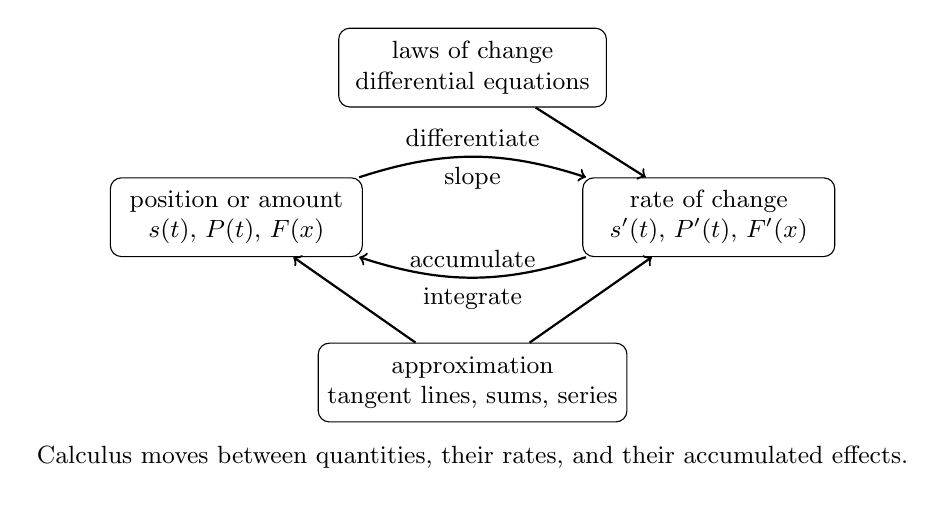
\begin{tikzpicture}[every node/.style={font=\small}]
\node[draw, rounded corners, align=center, minimum width=3.2cm, minimum height=1cm] (pos) at (0,0)
{position or amount\\ \(s(t)\), \(P(t)\), \(F(x)\)};

\node[draw, rounded corners, align=center, minimum width=3.2cm, minimum height=1cm] (vel) at (6,0)
{rate of change\\ \(s'(t)\), \(P'(t)\), \(F'(x)\)};

\node[draw, rounded corners, align=center, minimum width=3.4cm, minimum height=1cm] (approx) at (3,-2.1)
{approximation\\ tangent lines, sums, series};

\node[draw, rounded corners, align=center, minimum width=3.4cm, minimum height=1cm] (law) at (3,1.9)
{laws of change\\ differential equations};

\draw[->, thick] (pos) to[bend left=18] node[above] {differentiate} node[below] {slope} (vel);
\draw[->, thick] (vel) to[bend left=18] node[below] {integrate} node[above] {accumulate} (pos);

\draw[->, thick] (law) -- (vel);
\draw[->, thick] (approx) -- (pos);
\draw[->, thick] (approx) -- (vel);

\node at (3,-3.05) {Calculus moves between quantities, their rates, and their accumulated effects.};
\end{tikzpicture}
\caption{The main ideas of the book are connected from the beginning. The derivative measures local change. The integral accumulates change. Approximation makes both useful. Differential equations express laws in the language of change.}
\label{fig:first-map-of-calculus}
\end{figure}

This map is only a beginning. Two phrases still need a careful foundation: \(h\to0\)
and \(\text{better and better approximations by sums}.\)

Both depend on the same hidden idea: nearness. To make calculus honest, we need a precise language for numbers, intervals, functions, graphs, and limits. That language comes next.
\section{Discovery problems and projects}
\label{sec:chapter-one-discovery}

The dashboard story has given us four ways to talk about the same motion:

\[
\text{velocity},\qquad
\text{position},\qquad
\text{slope},\qquad
\text{signed area}.
\]

Before we build the formal language of limits, it is worth testing those ideas. The problems in this section are not only practice. They are small investigations. Each one asks you to read a graph, build a trip, or discover a pattern that will return later in a more precise form.

\subsection{Read a trip from a speed graph}
\label{subsec:read-trip-speed-graph}

The graph below records the velocity of a car over \(6\) hours. Velocity is measured in miles per hour. Positive velocity means the car moves in the chosen positive direction; negative velocity means it moves backward.

\begin{figure}[h]
\centering
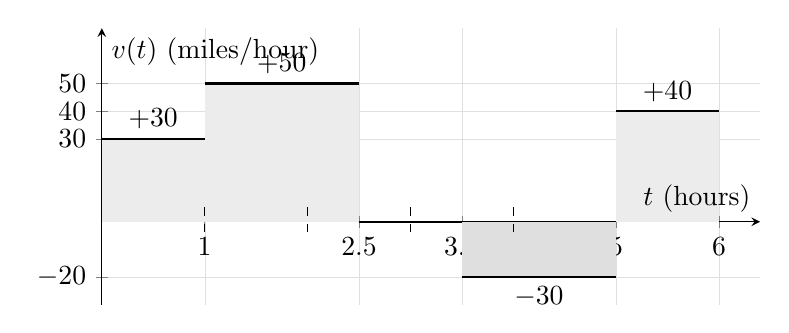
\begin{tikzpicture}
\begin{axis}[
    width=0.82\textwidth,
    height=0.42\textwidth,
    xmin=0, xmax=6.4,
    ymin=-30, ymax=70,
    axis lines=middle,
    xlabel={\(t\) (hours)},
    ylabel={\(v(t)\) (miles/hour)},
    xtick={0,1,2.5,3.5,5,6},
    xticklabels={\(0\),\(1\),\(2.5\),\(3.5\),\(5\),\(6\)},
    ytick={-20,0,30,40,50},
    grid=both,
    grid style={line width=.1pt, draw=gray!25},
]
\draw[fill=gray!15,draw=none] (axis cs:0,0) rectangle (axis cs:1,30);
\draw[fill=gray!15,draw=none] (axis cs:1,0) rectangle (axis cs:2.5,50);
\draw[fill=gray!25,draw=none] (axis cs:3.5,0) rectangle (axis cs:5,-20);
\draw[fill=gray!15,draw=none] (axis cs:5,0) rectangle (axis cs:6,40);

\addplot[thick] coordinates {(0,30) (1,30)};
\addplot[thick] coordinates {(1,50) (2.5,50)};
\addplot[thick] coordinates {(2.5,0) (3.5,0)};
\addplot[thick] coordinates {(3.5,-20) (5,-20)};
\addplot[thick] coordinates {(5,40) (6,40)};

\pgfplotsinvokeforeach{1,2,3,4}{
  \draw[dashed] (axis cs:#1,-3.8) -- (axis cs:#1,5.6);
}

\node[anchor=south] at (axis cs:0.5,30) {\(+30\)};
\node[anchor=south] at (axis cs:1.75,50) {\(+50\)};
\node[anchor=north] at (axis cs:4.25,-20) {\(-30\)};
\node[anchor=south] at (axis cs:5.5,40) {\(+40\)};
\end{axis}
\end{tikzpicture}
\caption{Each rectangle gives one signed change in position. Rectangles above the axis count positive; rectangles below the axis count negative.}
\label{fig:read-trip-speed-graph}
\end{figure}

\paragraph{Project.}
Starting from \(s(0)=0\), answer the following questions.

\begin{enumerate}
\item Compute the signed change in position on each time interval.
\item Fill in the position table:
\[
\begin{array}{c|cccccc}
t & 0 & 1 & 2.5 & 3.5 & 5 & 6 \\ \hline
s(t) & 0 & & & & &
\end{array}
\]
\item Sketch the graph of \(s(t)\). It should be made of straight line segments.
\item Find the displacement from \(t=0\) to \(t=6\).
\item Find the total distance traveled from \(t=0\) to \(t=6\).
\item Find the average velocity and the average speed over the whole trip.
\end{enumerate}

The signed rectangle areas are

\[
30\cdot 1,\qquad
50\cdot 1.5,\qquad
0\cdot 1,\qquad
(-20)\cdot 1.5,\qquad
40\cdot 1.
\]

Thus

\[
30+75+0-30+40=115.
\]

So the displacement is

\[
115\text{ miles}.
\]

The position table is

\[
\begin{array}{c|cccccc}
t & 0 & 1 & 2.5 & 3.5 & 5 & 6 \\ \hline
s(t) & 0 & 30 & 105 & 105 & 75 & 115
\end{array}
\]

The total distance traveled is different. For total distance, the backward part adds positively:

\[
30+75+0+30+40=155.
\]

Therefore

\[
\text{average velocity}
=
\frac{115}{6}\text{ miles/hour},
\]

while

\[
\text{average speed}
=
\frac{155}{6}\text{ miles/hour}.
\]

The same trip has two averages because displacement and distance traveled answer different questions.

\begin{quote}
Displacement asks: \emph{Where did you end compared with where you started?}

Distance traveled asks: \emph{How much road did you cover?}
\end{quote}

\subsection{Design two different trips with the same displacement}
\label{subsec:same-displacement-project}

A displacement is only a net result. It does not determine the whole trip.

Here are two different velocity histories on the interval \(0\leq t\leq 4\).

\[
v_A(t)=20
\]

and

\[
v_B(t)=
\begin{cases}
60, & 0\leq t<2,\\
-20, & 2<t\leq 4.
\end{cases}
\]

Both trips begin at \(s(0)=0\).

\begin{figure}[h]
\centering
\begin{minipage}{0.47\textwidth}
\centering
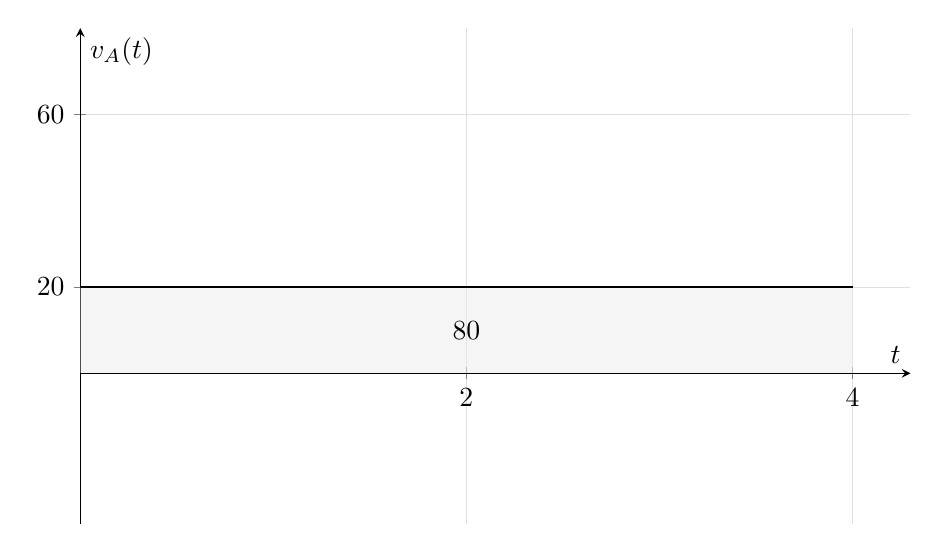
\begin{tikzpicture}
\begin{axis}[
    width=\textwidth,
    height=0.65\textwidth,
    xmin=0, xmax=4.3,
    ymin=-35, ymax=80,
    axis lines=middle,
    xlabel={\(t\)},
    ylabel={\(v_A(t)\)},
    xtick={0,2,4},
    ytick={0,20,60},
    grid=both,
    grid style={line width=.1pt, draw=gray!25},
]
\draw[fill=gray!15,draw=none,fill opacity=0.5] (axis cs:0,0) rectangle (axis cs:4,20);
\addplot[thick,domain=0:4,samples=2] {20};
\node at (axis cs:2,10) {\(80\)};
\end{axis}
\end{tikzpicture}

Trip A
\end{minipage}
\hfill
\begin{minipage}{0.47\textwidth}
\centering
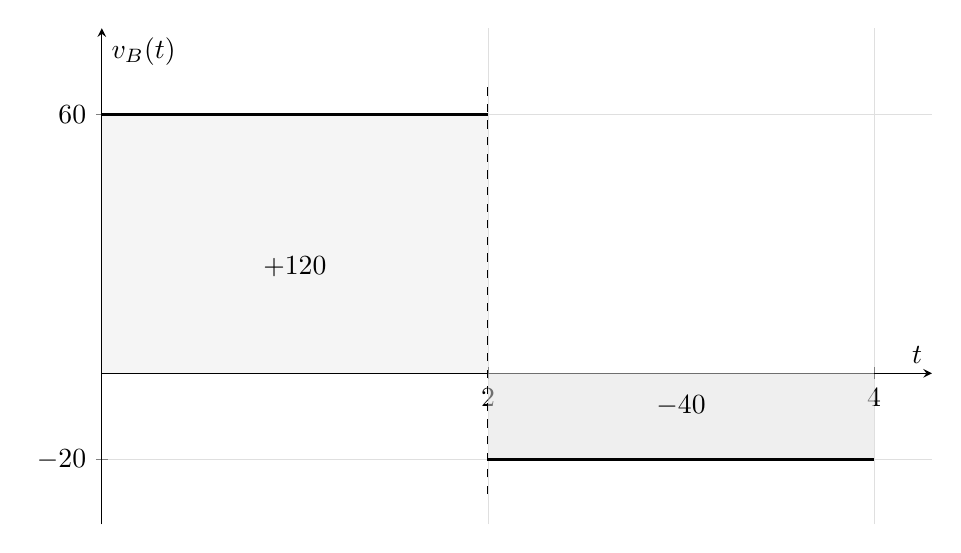
\begin{tikzpicture}
\begin{axis}[
    width=\textwidth,
    height=0.65\textwidth,
    xmin=0, xmax=4.3,
    ymin=-35, ymax=80,
    axis lines=middle,
    xlabel={\(t\)},
    ylabel={\(v_B(t)\)},
    xtick={0,2,4},
    ytick={-20,0,60},
    grid=both,
    grid style={line width=.1pt, draw=gray!25},
]
\draw[fill=gray!15,draw=none,fill opacity=0.5] (axis cs:0,0) rectangle (axis cs:2,60);
\draw[fill=gray!25,draw=none,fill opacity=0.5] (axis cs:2,0) rectangle (axis cs:4,-20);
\addplot[thick] coordinates {(0,60) (2,60)};
\addplot[thick] coordinates {(2,-20) (4,-20)};
\draw[dashed] (axis cs:2,-28) -- (axis cs:2,68);
\node[anchor=south] at (axis cs:1.0,20) {\(+120\)};
\node[anchor=north] at (axis cs:3,-3) {\(-40\)};
\end{axis}
\end{tikzpicture}

Trip B
\end{minipage}
\caption{Two different velocity histories can have the same displacement. Signed area preserves the net change, not the full story.}
\label{fig:same-displacement-two-trips}
\end{figure}

Trip A has displacement

\[
20\cdot 4=80.
\]

Trip B has displacement

\[
60\cdot 2+(-20)\cdot 2=120-40=80.
\]

So the final signed position is the same:

\[
s_A(4)=s_B(4)=80.
\]

But the total distance traveled is not the same. Trip A travels

\[
80
\]

miles. Trip B travels

\[
120+40=160
\]

miles.

\paragraph{Your turn.}
Design two new trips on \(0\leq t\leq 5\) that both have displacement \(100\) miles, but different total distances traveled.

One trip may use constant velocity. The other should include at least one interval of negative velocity.

Then answer:

\begin{enumerate}
\item What is the velocity function for each trip?
\item What is the displacement of each trip?
\item What is the total distance traveled by each trip?
\item Which graph gives a better story of what the driver actually did: the velocity graph or the final displacement alone?
\end{enumerate}

The last question matters. Calculus often compresses a whole history into one number. That number is useful, but it is not the whole story.

\subsection{Finite differences of squares and cubes}
\label{subsec:finite-differences-squares-cubes}

Finite differences already showed us the algebraic ancestor of calculus:

\[
\text{differences measure change},
\qquad
\text{sums rebuild accumulated change}.
\]

The square numbers gave the first famous pattern:

\[
0,\ 1,\ 4,\ 9,\ 16,\ 25,\ldots
\]

Their differences are

\[
1,\ 3,\ 5,\ 7,\ 9,\ldots
\]

because

\[
j^2-(j-1)^2=2j-1.
\]

Therefore

\[
\sum_{j=1}^{n}(2j-1)
=
\sum_{j=1}^{n}\bigl(j^2-(j-1)^2\bigr)
=
n^2.
\]

This is why the first \(n\) odd numbers add to a square:

\[
\boxed{1+3+5+\cdots+(2n-1)=n^2.}
\]

Now try cubes.

\[
\begin{array}{c|rrrrrr}
j & 0 & 1 & 2 & 3 & 4 & 5 \\ \hline
j^2 & 0 & 1 & 4 & 9 & 16 & 25 \\
\Delta(j^2) & & 1 & 3 & 5 & 7 & 9 \\[2mm]
j^3 & 0 & 1 & 8 & 27 & 64 & 125 \\
\Delta(j^3) & & 1 & 7 & 19 & 37 & 61
\end{array}
\]

The differences of cubes are not as simple as the differences of squares, but they still have a pattern.

\[
\Delta(j^3)=j^3-(j-1)^3.
\]

Expand:

\[
(j-1)^3=j^3-3j^2+3j-1.
\]

So

\[
\Delta(j^3)
=
j^3-(j^3-3j^2+3j-1)
=
3j^2-3j+1.
\]

Thus

\[
\boxed{\Delta(j^3)=3j^2-3j+1.}
\]

Now telescope:

\[
\sum_{j=1}^{n}\bigl(3j^2-3j+1\bigr)
=
\sum_{j=1}^{n}\bigl(j^3-(j-1)^3\bigr)
=
n^3.
\]

So

\[
\boxed{\sum_{j=1}^{n}\bigl(3j^2-3j+1\bigr)=n^3.}
\]

This identity can be used to discover a formula for the sum of squares. Let

\[
S_2(n)=1^2+2^2+\cdots+n^2.
\]

Also recall the formula

\[
1+2+\cdots+n=\frac{n(n+1)}{2}.
\]

From the cube difference identity,

\[
n^3
=
3\sum_{j=1}^{n}j^2
-
3\sum_{j=1}^{n}j
+
\sum_{j=1}^{n}1.
\]

That is,

\[
n^3
=
3S_2(n)
-
3\cdot \frac{n(n+1)}{2}
+
n.
\]

Solving for \(S_2(n)\),

\[
3S_2(n)
=
n^3+\frac{3n(n+1)}{2}-n.
\]

Put everything over \(2\):

\[
3S_2(n)
=
\frac{2n^3+3n^2+n}{2}
=
\frac{n(2n^2+3n+1)}{2}.
\]

Since

\[
2n^2+3n+1=(n+1)(2n+1),
\]

we get

\[
\boxed{
1^2+2^2+\cdots+n^2
=
\frac{n(n+1)(2n+1)}{6}.
}
\]

This formula did not appear from nowhere. It came from one idea:

\[
\text{differences telescope}.
\]

\paragraph{Discovery extension.}
Make a difference table for fourth powers:

\[
0^4,\ 1^4,\ 2^4,\ 3^4,\ 4^4,\ldots
\]

Then compute

\[
j^4-(j-1)^4.
\]

What kind of polynomial appears? What sum formula could it help you discover?

\subsection{A changing slope needs nearness}
\label{subsec:changing-slope-needs-nearness}

The finite examples in this chapter had flat velocity pieces and straight position pieces. Their slopes were easy to read.

Curved graphs force a sharper question.

For

\[
s(t)=t^2,
\]

the average velocity from \(t=2\) to \(t=2+h\) is

\[
\frac{s(2+h)-s(2)}{h}
=
\frac{(2+h)^2-4}{h}.
\]

For \(h\neq 0\),

\[
\frac{(2+h)^2-4}{h}
=
\frac{4+4h+h^2-4}{h}
=
4+h.
\]

So the nearby average velocities are

\[
4+h.
\]

They do not equal \(4\) unless \(h=0\), but \(h=0\) is not allowed in the fraction. Still, the closer \(h\) is to \(0\), the closer \(4+h\) is to \(4\).

The distance between the average velocity and \(4\) is

\[
|(4+h)-4|=|h|.
\]

So if we want the average velocity to be within \(0.01\) of \(4\), it is enough to require

\[
|h|<0.01.
\]

If we want it within \(0.0001\), it is enough to require

\[
|h|<0.0001.
\]

This is the first glimpse of the precise language of limits. A limit is not a guess from a table. It is a promise:

\[
\text{make the input close enough, and the output becomes as close as required.}
\]

For this example, the promise is easy because the error is exactly \(|h|\). In more difficult examples, the whole task is to control the error.

To do that carefully, we need a language for distance on the number line, intervals around a point, functions, graphs, and eventually limits. The next chapter builds that language. It may look like a review at first, but it is not a detour. It is the measuring tape calculus needs.
